\documentclass[a4paper,12pt]{article} % тип документа

% Поля страниц
\usepackage[left=2.5cm,right=2.5cm,
    top=2cm,bottom=2cm,bindingoffset=0cm]{geometry}
    
%Пакет дял таблиц   
\usepackage{multirow} 
    
%Отступ после заголовка    
\usepackage{indentfirst}


% Рисунки
\usepackage{floatrow,graphicx,calc}
\usepackage{wrapfig}

% Создаёем новый разделитель
\DeclareFloatSeparators{mysep}{\hspace{1cm}}

% Ссылки?
\usepackage{hyperref}
\usepackage[rgb]{xcolor}
\hypersetup{				% Гиперссылки
    colorlinks=true,       	% false: ссылки в рамках
	urlcolor=blue          % на URL
}


%  Русский язык
\usepackage[T2A]{fontenc}			% кодировка
\usepackage[utf8]{inputenc}			% кодировка исходного текста
\usepackage[english,russian]{babel}	% локализация и переносы


% Математика
\usepackage{amsmath,amsfonts,amssymb,amsthm,mathtools}


% Что-то 
\usepackage{wasysym}


\begin{document}


\begin{center}
\footnotesize{ФЕДЕРАЛЬНОЕ ГОСУДАРСТВЕННОЕ АВТОНОМНОЕ ОБРАЗОВАТЕЛЬНОЕ 			УЧРЕЖДЕНИЕ ВЫСШЕГО ОБРАЗОВАНИЯ}\\
\footnotesize{МОСКОВСКИЙ ФИЗИКО-ТЕХНИЧЕСКИЙ ИНСТИТУТ\\(НАЦИОНАЛЬНЫЙ 			ИССЛЕДОВАТЕЛЬСКИЙ УНИВЕРСИТЕТ)}\\
\footnotesize{ФАКУЛЬТЕТ ОБЩЕЙ И ПРИКЛАДНОЙ ФИЗИКИ\\}
\hfill \break
\hfill\break
\hfill\break
\hfill \break
\hfill \break
\hfill \break
\hfill \break
\hfill \break
\hfill \break
\hfill \break
\hfill \break
\hfill \break
\hfill \break
\hfill \break
\large{Лабораторная работа № 2.2.6\\\textbf{Определение энергии активации по температурной зависимости вязкости жидкости}}\\
\hfill \break
\hfill \break
\hfill \break
\begin{flushright}
	Серебренников Даниил\\
	Группа Б02-826
\end{flushright}
\hfill \break
\hfill \break
\hfill \break
\hfill \break
\hfill \break
\end{center}
\hfill \break
\hfill \break
\hfill \break
\hfill \break
\hfill \break
\hfill \break
\begin{center}
	Долгопрудный, 2019 г.
\end{center}
\thispagestyle{empty} % выключаем отображение номера для этой страницы


\newpage
	\textbf{Цель работы:} 1) измерение скорости падения шариков при разной температуре жидкости; 2) вычисление вязксоти жидкости по закону Стокса и расчет энергии активации.
	
	\textbf{В работе используются:} стеклянный цилиндр с исследуемой жидкостью (глицерин); термостат; секундомер; горизонтальный компаратор; микроскоп; мелкие шарики (диаметром 1-2 мм).
	
\section{Теоретическая часть}
\subsection{Энергия активации}
	Двойственный характер свойств жидкостей связан с особенностя- ми движения их молекул. В газах молекулы движутся хаотично, в их расположении отсутствует порядок. В кристаллических твердых телах частицы колеблются около определенных положений равновесия — узлов кристаллической решетки. В жидкостях, как и в кристал- лах, каждая молекула находится в потенциальной яме электрического поля, создаваемого окружающими молекулами. Молекулы колеблются со средней частотой, близкой к частоте колебаний атомов в кристаллических телах ($\sim 10^{12}$ Гц), и с амплитудой, определяемой размерами объема, предоставленного ей соседними молекулами. Глубина потенциальной ямы в жидкостях больше средней кинетической энергии колеблющейся молекулы, поэтому молекулы колеблются вокруг более или менее стабильных положений равновесия. Однако у жидкостей различие между этими двумя энергиями невелико, так что молекулы нередко выскакивают из <<своей>> потенциальной ямы и занимают место в другой.
	
	Для того чтобы перейти в новое состояние, молекула должна преодолеть участки с большой потенциальной энергией, превышающей среднюю тепловую энергию молекул. Для этого тепловая энергия молекул должна — вследствие флуктуации — увеличиться на некоторую величину $W$ , называемую энергией активации. Температурная зависимость вязкости жидкости при достаточно грубых предположениях можно опистаь формулой
	\begin{equation}
		\eta \sim A e^{W/kT}
	\end{equation}
	
\subsection{Формула Стокса}
	На всякое тело, двигающееся в вязкой жидкости, действует сила сопротивления. В общем случае величина этой силы зависит от многих факторов: от вязкости жидкости, от формы тела, от характера обтекания и т. д. Стоксом было получено строгое решение задачи о ламинарном обтекании шарика безграничной жидкостью. В этом случае сила сопротивления $F$ определяется формулой
	\begin{equation}
		F = 6\pi \eta r v
	\end{equation}
	
\subsection{Рассчетная формула вязкости}
	Измеряя на опыте установившуюся скорость падения шариков $v$ и величины $r$, $\rho$, $\rho_0$, можно определить вязкость жидкости по формуле
	\begin{equation}
		\label{formula}
		\eta = \frac{2}{9} g r^2 \frac{\rho - \rho_0}{v}
	\end{equation}
\section{Экспериментальная установка}
	Для измерений используется стеклянный цилиндрчиеский сосуд B, наполненный исследуемой жидкостью (глицерин). Диаметр сосуда $\approx 3$ см, длина $\approx 40$ см. На стенках сосуда нанесены две метки на некотором расстоянии друг от друга. Верхняя метка должна располагаться ниже уровня жидкости с таким расчетом, чтобы скорость шарика к моменту прохождения этой метки успевала установиться. Измеряя расстояние между метками с помощью линейки, а время падения с помощью секундомера, определяют скорость шарика vуст. Сам сосуд B помещен в рубашку D, омываемую водой из термостата. При работающем термостате температура воды в рубашке D, а потому и температура жидкости 12 равна температуре воды в термостате.
	
	Схема прибора (в разрезе) показана на рис.~\ref{ris:ustanovka}.
		\begin{figure}[H]
		\center{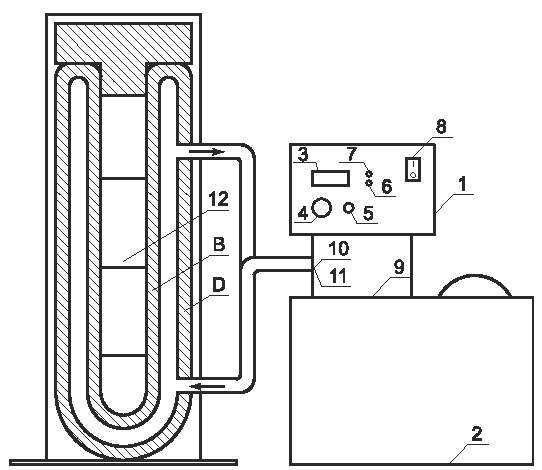
\includegraphics[scale=1]{Ustanovka.pdf}}
		\caption{Установка для определения коэффициента вязкости жидкости.}
		\label{ris:ustanovka}
	\end{figure} 
\section{Модель экспермиента}
	\begin{enumerate}
		\item Отберем 20 шариков различного диаметра и с помощью микроскопа измерим их средние диаметры
		\item Измерим установившиеся скорости падения шариков и вычислим вязкость по формуле (\ref{formula}). Измерения выполним для 7 значений температуры в интервале от 25-55$^\circ$C.
		\item Для каждого из опытов вычислим значение числа Рейнольдса $Re$, оценим время релаксации $\tau$ и путь релаксации $S$. Проанализируем применимость формулы Стокса в каждом эксперименте.
		\item Построим график зависимости $\ln{\eta / \eta_0}$ от $1/T$.
		\item По угловому коэффициенту прямой $\ln{\eta / \eta_0} (1/T)$ определим энергию активации $W$.
		\item Оценим погрешность полученных результатов.
	\end{enumerate}



\newpage
\section{Экспериментальные данные}
	В таблице~\ref{table:const} приведены константы, используемые в лабораторной работе.
	
	\floatsetup[table]{capposition=top}	
	\begin{table}[H]
		\caption{Постоянные величины.}
		\label{table:const}
\begin{tabular}{|c|c|c|c|}
	\hline
	\begin{tabular}[c]{@{}c@{}}Плотность\\ этанола\\ $\rho_0$, кг/м$^3$\end{tabular} & \begin{tabular}[c]{@{}c@{}}Плотность\\ воды\\ $\rho$, кг/м$^3$\end{tabular} & \begin{tabular}[c]{@{}c@{}}Ускорение свободного падения\\ $g$, м/c$^2$\end{tabular} & \begin{tabular}[c]{@{}c@{}}Пересчетный коэффициент\\ микроманометра\\ $k$\end{tabular} \\ \hline
	809,5                                                                            & 1000,0                                                                      & 9,81                                                                                & 0,2                                                                                    \\ \hline
\end{tabular}
	\end{table}
	
	В следующих таблицах~\ref{table:glass_n}~-~\ref{table:Fe_n} представлены результаты измерений и вычислений физических величин, значения которых необходимы для анализа прмиенимости формулы Стокса в каждом эксперименте.
\floatsetup[table]{capposition=top}	
	\begin{table}[H]
		\caption{Стеклянный шарик.}
		\label{table:glass_n}
\begin{tabular}{|c|c|c|c|c|c|c|c|c|}
\hline
$T$, K & $t_1$, с & $t_2$, с & $d$, мм & $\eta$, мПа$\cdot$c & $\sigma_\eta$, мПа$\cdot$c & $Re$   & $\tau$, мс & $S$, мм \\ \hline
297,8  & 26,16    & 52,72    & 2,06    & 770                 & 40                         & 0,0063 & 0,8        & 2,9     \\ \hline
303,3  & 23,06    & 46       & 2,06    & 660                 & 30                         & 0,0085 & 0,94       & 3,8     \\ \hline
308,2  & 17,69    & 34,4     & 2,08    & 490                 & 20                         & 0,0159 & 1,2        & 7,3     \\ \hline
313,2  & 11,68    & 23,25    & 2,04    & 326                 & 16                         & 0,0340 & 1,8        & 15      \\ \hline
318,2  & 9,56     & 17,06    & 2,2     & 245                 & 11                         & 0,0754 & 2,7        & 36      \\ \hline
328    & 4,38     & 8,74     & 2,1     & 129                 & 6                          & 0,2356 & 4,7        & 108     \\ \hline
\end{tabular}
	\end{table}		

	\floatsetup[table]{capposition=top}	
	\begin{table}[H]
		\caption{Железный шарик.}
		\label{table:Fe_n}
\begin{tabular}{|c|c|c|c|c|c|c|c|c|}
\hline
$T$, K & $t_1$, с & $t_2$, с & $d$, мм & $\eta$, мПа$\cdot$c & $\sigma_\eta$, мПа$\cdot$c & $Re$   & $\tau$, мс & $S$, мм \\ \hline
297,9  & 29,52    & 59,91    & 0,84    & 770                 & 90                         & 0,0022 & 0,4        & 1,3     \\ \hline
303,3  & 22,08    & 43,94    & 0,92    & 660                 & 70                         & 0,0040 & 0,6        & 2,5     \\ \hline
308,2  & 18,74    & 37,2     & 0,84    & 470                 & 60                         & 0,0061 & 7          & 3,5     \\ \hline
313,2  & 12,43    & 25,36    & 0,9     & 380                 & 40                         & 0,0116 & 0,9        & 7,1     \\ \hline
318,1  & 7,73     & 15,27    & 0,9     & 220                 & 20                         & 0,0343 & 1,6        & 21      \\ \hline
323,1  & 5,72     & 11,3     & 0,88    & 155                 & 18                         & 0,0642 & 2,2        & 38      \\ \hline
328,0  & 4,07     & 8,26     & 0,9     & 122                 & 14                         & 0,1120 & 2,9        & 68      \\ \hline
\end{tabular}
	\end{table}
		
	На рис.~\ref{ris:Graph_1} изображен график зависимости $\ln{\eta / \eta_0}$ от $1 / T$, где $\eta_0 = 1480$ мПа$\cdot$с - табличное значение вязкости глицерина при $T = 293$ К.


	
\newpage
		\begin{figure}[H]
		\center{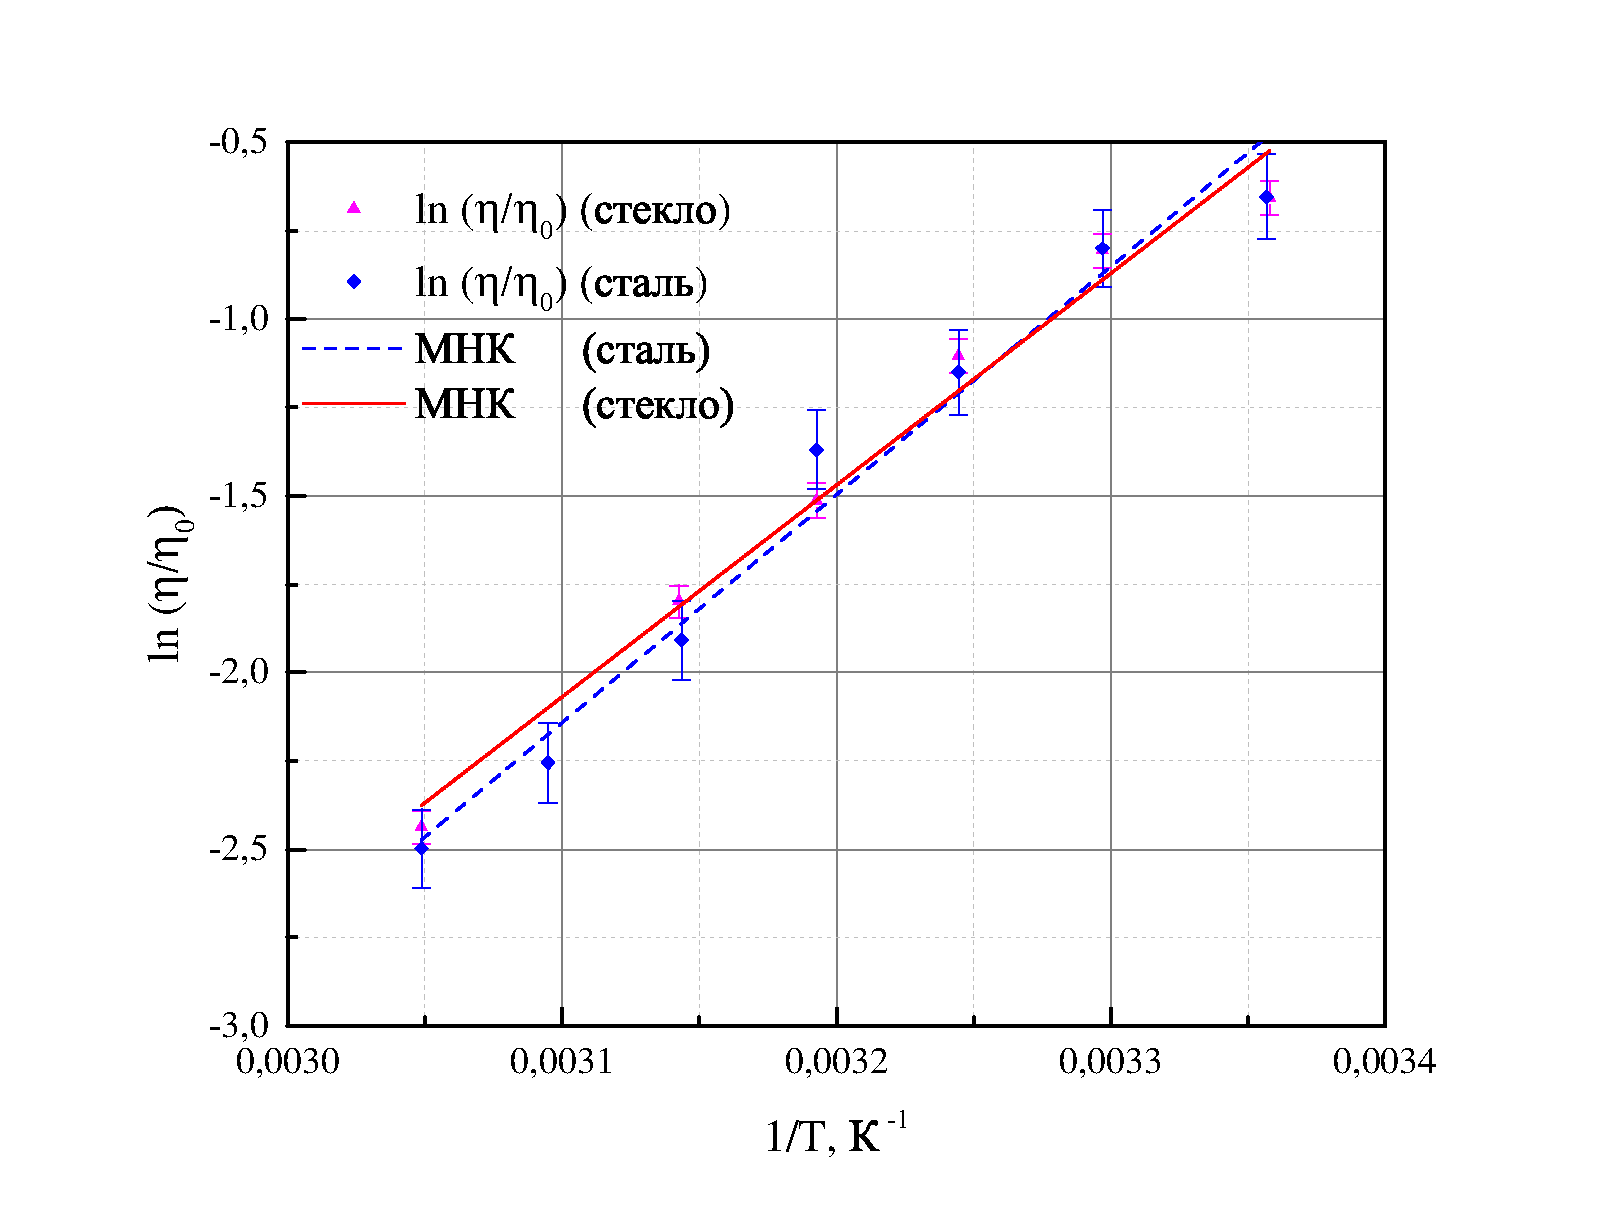
\includegraphics[scale=0.5]{Graph_1.pdf}}
		\caption{Зависимость $\ln{\eta / \eta_0}$ от $1 / T$.}
		\label{ris:Graph_1}
	\end{figure}
	
	Наклоном графика (рис.~\ref{ris:Graph_1}) будет являться величина $W/k$. Значения экспериментальных точек и значение энергии активации представлены в таблицах~\ref{table:glass_W} -~\ref{table:Fe_W}.
	
\floatsetup[table]{capposition=top}	
	\begin{table}[H]
		\caption{Стеклянный шарик.}
		\label{table:glass_W}
\begin{tabular}{|c|c|c|c|c|c|}
\hline
$1/T$, К$^{-1}$ & $\ln{\eta/\eta_0}$ & $\sigma_{\ln{\eta/\eta_0}}$ & $W/k$, К              & $W$, зДж            & $\sigma_W$, зДж    \\ \hline
0,00336         & -0,66              & 0,05                        & \multirow{6}{*}{6000} & \multirow{6}{*}{83} & \multirow{6}{*}{5} \\ \cline{1-3}
0,0033          & -0,81              & 0,05                        &                       &                     &                    \\ \cline{1-3}
0,00324         & -1,11              & 0,05                        &                       &                     &                    \\ \cline{1-3}
0,00319         & -1,51              & 0,05                        &                       &                     &                    \\ \cline{1-3}
0,00314         & -1,80              & 0,05                        &                       &                     &                    \\ \cline{1-3}
0,00305         & -2,44              & 0,05                        &                       &                     &                    \\ \hline
\end{tabular}
	\end{table}	
	
\floatsetup[table]{capposition=top}	
	\begin{table}[H]
		\caption{Железный шарик.}
		\label{table:Fe_W}
\begin{tabular}{|c|c|c|c|c|c|}
\hline
$1/T$, К$^{-1}$ & $\ln{\eta/\eta_0}$ & $\sigma_{\ln{\eta/\eta_0}}$ & $W/k$, К              & $W$, зДж            & $\sigma_W$, зДж    \\ \hline
0,00336         & -0,65              & 0,12                        & \multirow{7}{*}{6400} & \multirow{7}{*}{89} & \multirow{7}{*}{7} \\ \cline{1-3}
0,0033          & -0,80              & 0,11                        &                       &                     &                    \\ \cline{1-3}
0,00324         & -1,15              & 0,12                        &                       &                     &                    \\ \cline{1-3}
0,00319         & -1,37              & 0,11                        &                       &                     &                    \\ \cline{1-3}
0,00314         & -1,91              & 0,11                        &                       &                     &                    \\ \cline{1-3}
0,0031          & -2,26              & 0,11                        &                       &                     &                    \\ \cline{1-3}
0,00305         & -2,50              & 0,11                        &                       &                     &                    \\ \hline
\end{tabular}
	\end{table}

\newpage	
\section{Обсуждение результатов}	
	Обсуждение результатов хотелось бы начать с анализа формулы Стокса. В каждом опыте значение числа Рейнольдса $Re$ было очень маленьким (меньше $0.5$), поэтому можно считать, что обтекание шарика жидкостью действительно имело ламинарный характер и формула Стокса праведлива в данной лабораторной работе. Более того, время релаксации $\tau < t_1$ и путь релаксации $S < l$ в каждом из опытов, поэтому от второй до третьей отметки шарики однозначно двигались с установившейя скоростью. Значения вязкости в каждом из опытов или совпадают с табличными значениями в пределах погрешности, или незначительно отличаются. При $T = 298$К вязкость 99\% водного раствора глицерина $\eta = 772$ мПа$\cdot$c, а при $T = 303$К вязкость 100\% водного раствора глицерина $\eta = 662$ мПа$\cdot$c, исходя из этих данных, можно заключить, что у исследуемой нами жидкости весовой процент глицерина равен 99 - 100\%.
	
	Наибольший интерес представляет собой анализ конечного результата энергии активации $W$ - энергии, приходящейся на одну молекулу глицерина для преодолевания потенциального барьера, препятствующего занять <<соседнее положение равновесия>>. Рассчитаем энергию, приходящую на один моль глицерина $w = W N_A$. Для рассчета воспользуемся значением энергии активации, полученным при анализе графика зависимости $\ln{\eta / \eta_0}$ от $1 / T$ для стальных шариков $w \approx 54$ кДж/моль. Можно предположить, что перемещение молекулы в <<другую>> потенциальную яму может произойти благодаря разрыву химических связей с соседними молекулами. Глицерин $\mathrm{C_3 H_5 (OH)_3}$ -- простейший представитель трёхатомных спиртов, в которых естественным образом возникают межмолекулярные водородные связи. Действительно, следствием полярности связи $\mathrm{O \! - \! H}$ и наличия неподеленных электронных пар на атоме кислорода является способность гидроксосоединений к образованию водородных связей. Среднее табличное значение энергии водородной связи $\mathrm{O \! \cdot \cdot \cdot \! H}$ $w_0 = 20$ кДж/моль. Грубой оценкой $w / w_0$ получается, что в среднем одна молекула глицерина образует 3 водородные связи. Однако,рассматривая пространственную структуру молекулы глицерина, можно сказать, что она может образовать больше 3 водородных связей. Является ли наше предположение о том, на что идёт энергия активация ошибочным? Конечно, нет. Ведь можно ожидать, что энергия активации молекулы близка к энергии кипения жидкости, приходящейся на одну молекулу, которая однозначно связана с разрывом водородных связей. Табличное значение $\Delta H = 61$ кДж/моль, откуда следует, что на 1 молекулу глицерина в среднем приходится 3 водородные связи.
	
\section*{Выводы}
	\begin{itemize}
		\item Проверили справедливость закона Стокса в условиях эксперимента.
		\item Вычислили вязкость исследуемой жидкости по закону Стокса, например при $T = 298$ К $\eta = (770\, \pm \, 40)$ мПа$\cdot$с, что соотвествует табличному значению 99\% раствора глицерина.
		\item Вычислили энергию активации глицерина $W =(89 \, \pm \, 7)$ зДж.
		\item Оценили сколько в среднем водородных связей приходится на одну молекулу глицерина --~3.
	\end{itemize}
	
	
	
	
	
	
	
	
	
	
	
	
	
	
	
	
	
	
	
	
	
	
	
	
	
	
	
	
	
	
	















\end{document}